%!TEX encoding = UTF-8 Unicode
\subsection{Shuttle}
\label{subsec:Architecture}
%- Como pensam abordar a tese tendo em conta o problema, as contribuicoes a que propoe a dar e a arquitectura definida.
%- Descricao de alto nivel da arquitectura do sistema: Arquitectura do SW explicando os principais componentes e as funcoes que executam.
%- Como procederam as escolhas das ferramentas, linguagens de programcao, ambientes de desenvolvimento, hardware
%- Como prevem desenvolver a arquitectura proposta: por onde vao comecar. Como vao integrar os componentes, que dificuldades esperam encontrar e que estrategias planeam para as ultrapassar.
%%%%%%%%%%%%%%%%%%%%%%%%%%%%%%%%%%%%%%%%%%

%%Caracteristicas: contribuicoes, escolhas e challenges
Shuttle is an intrusion recovery service for PaaS. It recovers from intrusions on software domain due to software flaws, corrupted requests, input mistakes, corrupted data and suspicious intrusions in PaaS containers. While previous works aimed to perform intrusion recovery in applications with a single database, Shuttle targets PaaS applications which are deployed in multiple containers and backed by SQL or NoSQL databases. Since typical PaaS applications are designed to support high usage loads, our main contribution is a scalable intrusion recovery service which is transparent for application developers. Shuttle logs and replays user HTTP requests to recover from intrusions.

% System Modules 
Our service is designed using a proxy architecture that logs the user HTTP requests without modification of PaaS components. Shuttle is composed of the following modules (Figure \ref{architecture}): 
\begin{itemize}
  \item \textbf{Proxy:} The HTTP proxy logs all user HTTP requests, adds a timestamp mark to their header and forwards them to the load balancer.
  \item \textbf{Load balancer:} The load balancer, which is part of the PaaS system, spreads the requests through the web servers according to their usage. 
  \item \textbf{Web servers:} The application-logic tier composed by HTTP web servers deployed in PaaS containers. The applications access the database through a provided PaaS service. The service contains a \textbf{database client auditor} which logs the accessed data items per request. 
  \item \textbf{Database instances:} The database tier is a single relational database instance or a set of instances running a NoSQL database software that stores the application persistent state. Each instance is deployed in a container and has a \textbf{database server auditor} which logs the requests which accessed each data item.
  \item \textbf{Request storage:} A scalable storage system which stores the requests, the responses and their metadata.
  \item \textbf{Replay instances:} The replay instances are HTTP clients that read previous requests from the requests storage and send them to the web servers for being re-execute during the recovery phase. These worker instances are coordinated by the manager.
  \item \textbf{Manager:} The manager retrieves the dependencies and coordinates the replay and database instances. 
\end{itemize}


\begin{figure}
  \centering
  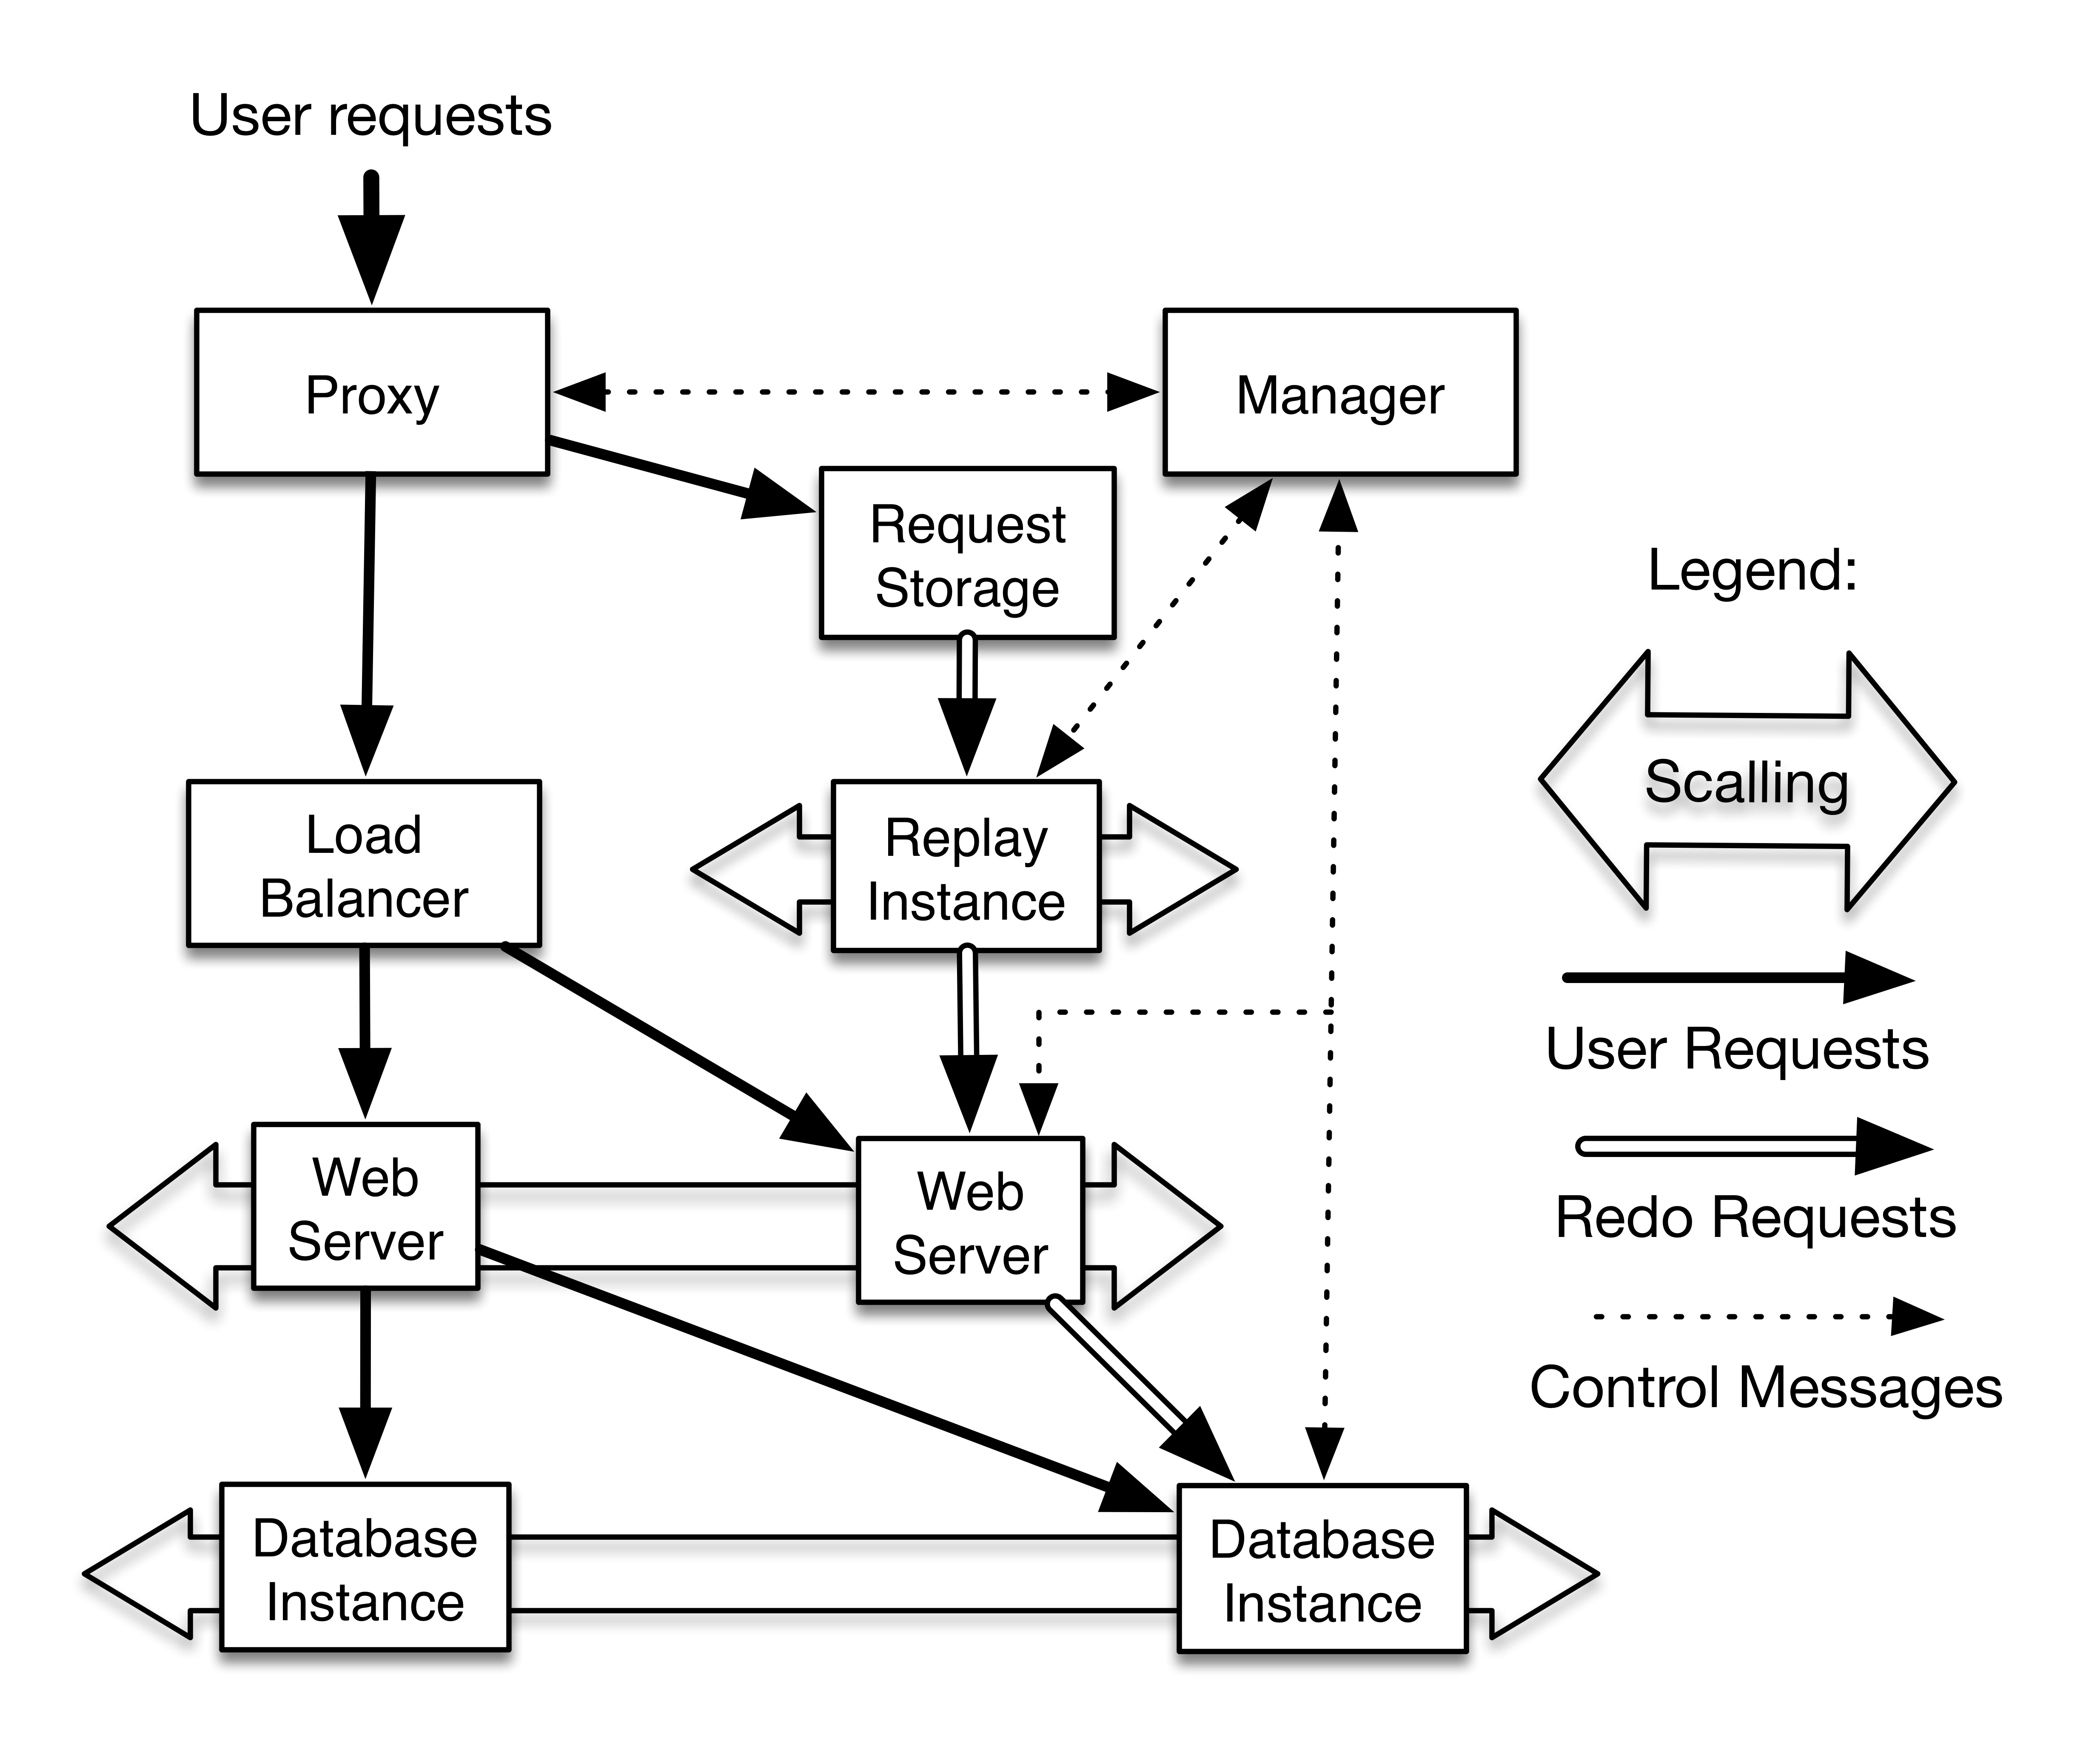
\includegraphics[width=90mm]{images/architectureTiers}
  \caption{Overview of the proposed service}
  \label{architecture}
\end{figure}

Shuttle leverages the transparency and elasticity of PaaS systems. Shuttle uses the PaaS controller to deploy an array of replay containers. Most of PaaS systems scale automatically and horizontally, i.e., they increment or decrement the number of containers based on the measurements of the containers usage. Therefore, the application-logic and data tiers scale to attend the requests from the replay containers, increasing the recovery speed. More, PaaS systems include a load balancer and nearly all deployed applications use HTTP protocol. Finally, most developers use a provided storage service, which can hide the Shuttle service.\\

%Which kind of faults? How they are detected? How they are fixed?
Shuttle recovers from software flaws faults and interaction faults from input mistakes, attacks and intrusions. To do so, Shuttle has two phases: record and replay. 

%Como e que o Shuttle vai fazer o recovery
During the record phase, the \textit{proxy} logs the user HTTP requests, adds a timestamp to its header as request id and forwards them to the load balancer. These requests are stored in an external distributed storage system using asynchronous I/O, which permits the request to proceed before the transmission has finished. After being forward by the load balancer, each request is attended by a web server. The database client auditor, deployed in each web server, logs the accessed database items. 
Each database instance has a database server auditor which intercepts the database accesses. The auditor records the client request timestamp and serializes the access to each data item, allowing multiple-reads or a single write. The access sequence of each data item is sent to the \textit{manager} to generate the dependency graph. At the end, the response is also stored in the external storage.
In summary, the external storage contains the request, response and accessed data items and the manager retrieves the accessed data items to generate the dependency graph.

%% - Replay phase
The replay phase is initialized when intrusions are detected or the application software requires an update. The detection of the fault is out of the scope of this work. In order to fix the exploited vulnerabilities, Shuttle supports software updates in the application or database instances. More, it supports the modification of user requests to remove accidental or malicious behaves. Then the \textit{manager} initiates new PaaS containers, which may include code fixes, and loads the snapshot on each database instance. The new application containers are intrusion-less because the snapshot is previous to the intrusion and the containers are renewed to include vulnerability patches. After, the requests are replayed in parallel using a set of \textit{replay containers}. The replayed requests access the database version loaded in the new containers. Since users still use the corrupted computation containers and database, the application remains online, perhaps with a degraded behavior, without exposing downtime to users. After recovery, the user requests are switched to the application with fixed state.\\


%-------------------------------------------------
The first version of Shuttle will replay every user request \cite{undoForOperators}. We assume that critical software flaws and intrusions can be detected in a short period of time, from seconds to one week. If a fault exists during a long period then the application may tolerate a longer recovery phase because the recovery process does not require application downtime. A future work may concern to perform selective replay using taint propagation via replay \cite{warp}. Still, one of the main challenges of Shuttle is to reduce the recovery time. To do so, we use two techniques: snapshot (See Section \ref{subSec:RecoveryModels}) and parallel replay.

Performing snapshots in distributed NoSQL databases (DynamoDB \cite{Decandia2007}, Bigtable \cite{Chang2008}) is not trivial since they have to be consistent with the computation tier user requests. User requests may include multiple database accesses, each of them to multiple database servers. The snapshots have to include only completed user requests. Otherwise the replay phase will be inconsistent if Shuttle replays the requests in a snapshot that contains part of the persistent state written during the previous execution of the replayed requests. Therefore, the \textit{manager} leverages the request timestamping to schedule a snapshot. The administrator defines a future instant in time, $t$, where the snapshot will occur and the manager forwards this information to every database instance. The requests, which have a timestamp bigger than $t$, write to a new version and read the latest version. The remain requests write to the previous version and read only the versions written by requests with timestamp lower than $t$. This mechanism is based on copy-on-write mechanisms.\\

To support runtime-recovery, the snapshot is loaded in a new branch, similar to the model used by git \cite{git}. The branch isolation allows multiple, perhaps simultaneous, replay attempts without compromising the exposed application behavior. More, it allows developers to test software updates with real data or discard a recovery process. To do so, the manager defines the branch used by the new user requests and by the requests which are being replayed.\\ 

Previous proposals \cite{Akkus2010} leverage the request serialization provided by snapshot isolation in relational DBMS to sort the replay operations. However, PaaS applications perform multiple \textit{transactions} accessing independent data items in NoSQL database instances. Therefore, we need a new approach to serialize the requests and the data item accesses during the replay phase. More, the data items accessed during the replay phase may change due to code updates, request modification or multi-threaded execution. While \textit{Undo for Operators} \cite{undoForOperators} uses the application protocol knowledge to establish the dependency between requests, our work aims to support any application deployed on PaaS. Therefore, we use the captured database data item access list to generate a dependency graph. The graph reflects the dependencies between requests during their execution. False dependencies in the graph do not cause data loss or inconsistent state since they are used only to order the requests replay as \textit{in} \cite{Ammann2002}.

Shuttle can not execute requests in serial order. It would not have only performance degradation but also lock the replay phase because the requests are originally executed in parallel and may depend from each other. On the other hand, PaaS applications have loosely coupled requests that share data only by data items in the database. Therefore, Shuttle will perform as many requests in parallel as possible to reduce the duration of the replay phase. The PaaS controller will auto-scale the database and application-logic tiers adding more containers. More, Shuttle manager can request the PaaS controller to initiate multiple replay containers to increase the replay performance. 
Yet, the user requests are processed in parallel using multi-threaded servers and the system messages, including the database requests, do not have a delivering order. With this in mind, Shuttle uses the access list per data item to record and to order the accesses to each data item. This method is dead-lock free if the code and requests remain equal to the original execution. Otherwise, some request may not access the same sequence of data items or read/write the same content during the replay phase creating request starvation and locking the replay process. Therefore, the database client interceptors will fetch the list of data items accessed by the original request execution and simulate the access to the remaining data items to unlock their remaining requests.\\

There are four main sources of non-determinism in each application server: concurrent threads, random number generation, time accesses and requests order. The concurrent threads are ordered using the database access mechanisms, which were introduced above. To solve the remaining issues, the \textit{proxy} adds pseudo-random number generator seed and its timestamp (also used as request ID) to the request header. Application developers can access these non-deterministic variables in a deterministic way using the PaaS middleware API. This mechanism is language independent. Despite the fact it just returns one timestamp per request, we argue that it is acceptable for most applications. \\ 

The elected database to backend the prototype is the key-value storage Voldemort \cite{Kreps}. Voldemort is an open source implementation of Amazon Dynamo DB \cite{Decandia2007} in use by Linkedin \cite{linkedin}. Key-value storage databases are common in PaaS environments because they scale properly and provide a simple put, get, delete API. We leverage the API simplicity to avoid delays and mistakes of parsing SQL queries \cite{phoenix}. More, Voldemort provides to the applications the capability of resolve the conflicts by choosing the best suited data item version. We may leverage this characteristic to solve replay conflicts and application integrity issues. \\

The external users requests and responses will be stored in the scalable NoSQL database Cassandra \cite{Lakshman2010a}. The database can be replicated to a remote site to prevent catastrophic disasters. The database server auditor can be implemented as a proxy. Shuttle uses the externally stored user requests to recover from any kind of intrusion in the computation and database instances. Since PaaS defines containers to run applications, Shuttle will collaborate with the coordinator of the PaaS system to lunch new containers using intrusion-free container images, which may include software updates. The software updates can prevent future intrusions or fix a discovered flaw \cite{Wang2011,warp}. The old containers, which may contain unknown intrusions or a corrupted operating system, are shutdown. Shuttle updates the application persistent state to be coherent with the new software version. Shuttle leverages the pay-per-usage model of PaaS to provide a cost-efficient and fast recovery service.


By replaying the user requests in parallel using intrusion-free PaaS containers and a clean database snapshot, we aim to recover from security intrusions in PaaS applications.
